\documentclass[tikz,border=10pt]{standalone}
\usetikzlibrary{positioning, arrows.meta, shapes.geometric, decorations.pathreplacing, calc}

\begin{document}
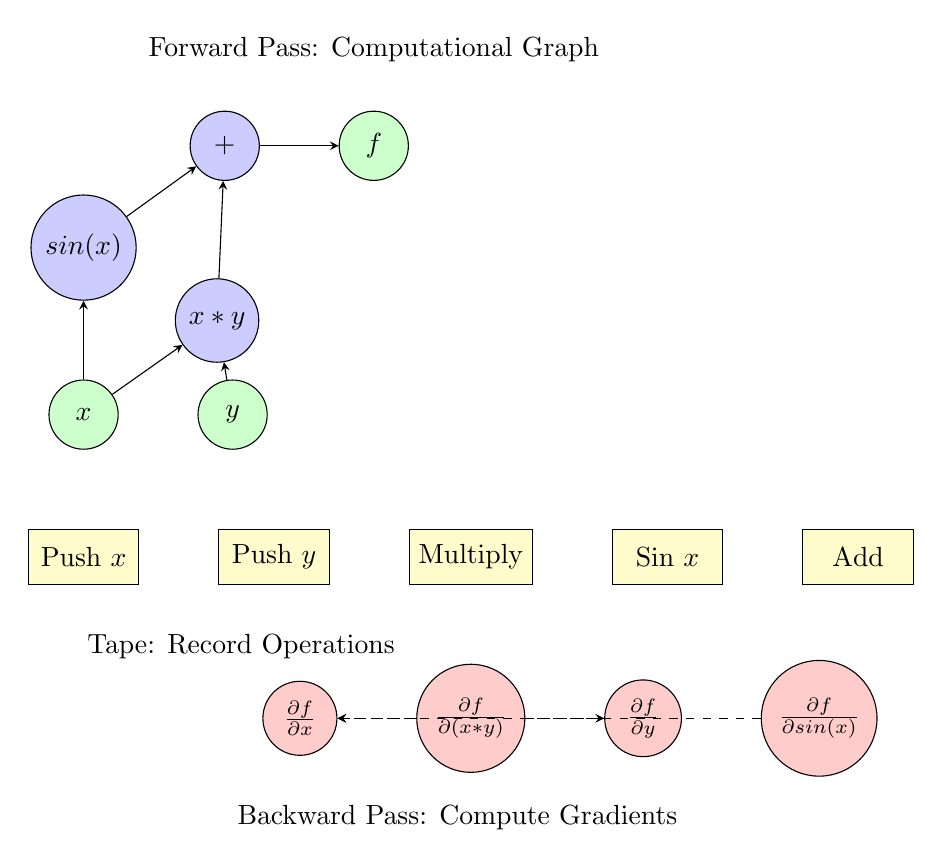
\begin{tikzpicture}[
    opnode/.style={circle, draw, fill=blue!20, minimum size=25pt},
    varnode/.style={circle, draw, fill=green!20, minimum size=25pt},
    gradient/.style={circle, draw, fill=red!20, minimum size=25pt},
    arrowstyle/.style={->,>=stealth},
    tapestyle/.style={draw, fill=yellow!20, minimum height=20pt, minimum width=40pt, align=center}
]

% Forward pass nodes
\node[varnode] (x) {$x$};
\node[varnode, right=of x] (y) {$y$};
\node[opnode, above right=of x, yshift=-0.5cm] (mult) {$x*y$};
\node[opnode, above=of x] (sin) {$sin(x)$};
\node[opnode, above right=of sin, yshift=-0.5cm] (sum) {$+$};
\node[varnode, right=of sum] (f) {$f$};

% Forward pass arrows
\draw[arrowstyle] (x) -- (mult);
\draw[arrowstyle] (y) -- (mult);
\draw[arrowstyle] (mult) -- (sum);
\draw[arrowstyle] (x) -- (sin);
\draw[arrowstyle] (sin) -- (sum);
\draw[arrowstyle] (sum) -- (f);

% Tape
\node[tapestyle, below=of x] (tapex) {Push $x$};
\node[tapestyle, right=of tapex] (tapey) {Push $y$};
\node[tapestyle, right=of tapey] (tapemult) {Multiply};
\node[tapestyle, right=of tapemult] (tapesin) {Sin $x$};
\node[tapestyle, right=of tapesin] (tapesum) {Add};

% Backward pass (gradients)
\node[gradient, below=of tapemult] (gmult) {$\frac{\partial f}{\partial (x*y)}$};
\node[gradient, left=of gmult] (gx) {$\frac{\partial f}{\partial x}$};
\node[gradient, right=of gmult] (gy) {$\frac{\partial f}{\partial y}$};
\node[gradient, right=of gy] (gsin) {$\frac{\partial f}{\partial sin(x)}$};

% Backward pass arrows
\draw[arrowstyle, dashed] (gmult) -- (gx) node[midway, above] {};
\draw[arrowstyle, dashed] (gmult) -- (gy) node[midway, above] {};
\draw[arrowstyle, dashed] (gsin) -- (gx) node[midway, above] {};

% Annotations
\node[above=0.5cm of f] (forwardlabel) {Forward Pass: Computational Graph};
\node[below=0.5cm of tapex, xshift=2cm] (tapelabel) {Tape: Record Operations};
\node[below=0.5cm of gx, xshift=2cm] (backwardlabel) {Backward Pass: Compute Gradients};

\end{tikzpicture}
\end{document}
